\documentclass[usenames,dvipsnames,handout]{beamer}

\usepackage{tikz}
\usepackage{tkz-berge}
\usepackage{tkz-graph}
\usepackage{subcaption}

\usetikzlibrary{patterns,arrows,decorations.pathreplacing}

\usepackage{xcolor}
\definecolor{dblue}{RGB}{20,66,129}
\definecolor{rose}{RGB}{255,101,122}
\definecolor{crimsonred}{RGB}{132,22,23}
\definecolor{darkblue}{RGB}{72,61,139}

\definecolor{deepblue}{RGB}{36,123,160}
\definecolor{deepred}{RGB}{255,22,84}
\definecolor{deeporange}{RGB}{240,111,62}

\definecolor{olive}{rgb}{0.3, 0.4, .1}
\definecolor{fore}{RGB}{249,242,215}
\definecolor{back}{RGB}{51,51,51}
\definecolor{title}{RGB}{255,0,90}
\definecolor{dgreen}{rgb}{0.,0.6,0.}
\definecolor{gold}{rgb}{1.,0.84,0.}
\definecolor{JungleGreen}{cmyk}{0.99,0,0.52,0}
\definecolor{BlueGreen}{cmyk}{0.85,0,0.33,0}
\definecolor{RawSienna}{cmyk}{0,0.72,1,0.45}
\definecolor{Magenta}{cmyk}{0,1,0,0}


\usecolortheme[named=Red]{structure} 

\DeclareMathOperator{\RR}{\textbf{R}}
\DeclareMathOperator{\QQ}{\textbf{Q}}
\DeclareMathOperator{\ZZ}{\textbf{Z}}
\DeclareMathOperator{\fordim}{\text{dim}_{\textbf{F}}}
\DeclareMathOperator{\hausdim}{\text{dim}_{\textbf{H}}}
\DeclareMathOperator{\minkdim}{\text{dim}_{\textbf{M}}}

%\usecolortheme{beaver}




\title{Salem Sets Avoiding Patterns}
\author{Jacob Denson\\The University of Wisconsin-Madison}
\institute{}

\begin{document}

\maketitle






\begin{frame}
    \ 
\end{frame}




\begin{frame}
    \frametitle{General Research Question}

    \begin{center}
    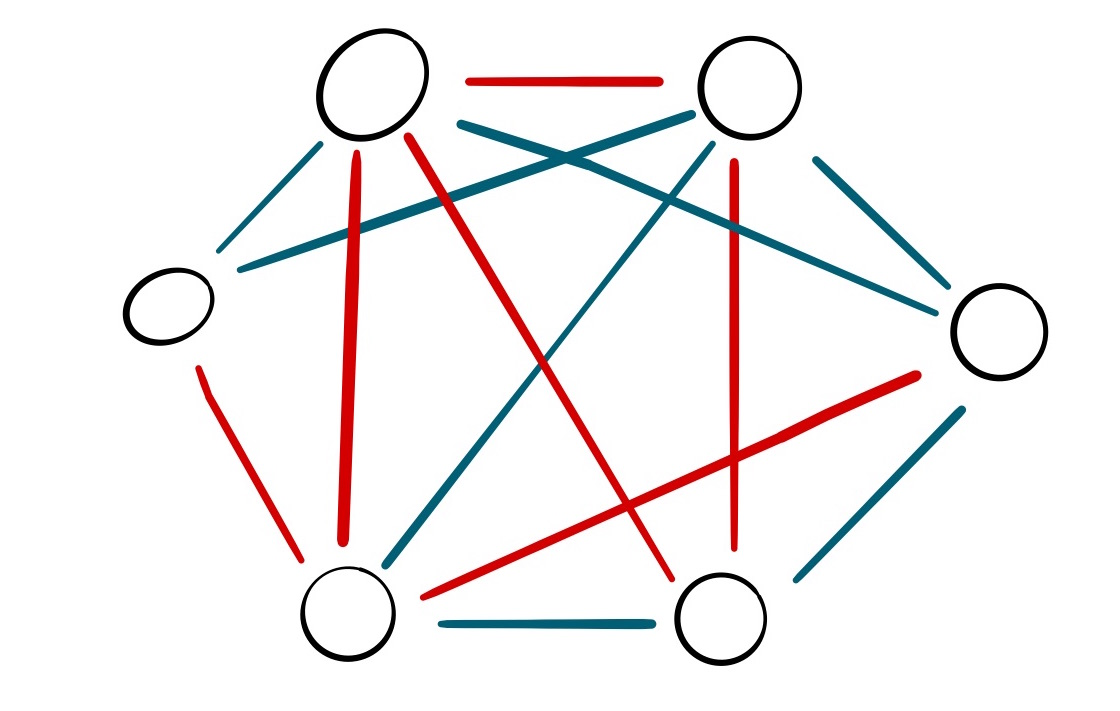
\includegraphics[width=0.4\textwidth]{../Images/RamseyTheory}
    \end{center}

    \begin{itemize}
        \item Phenomenon: Structure appears in suitably large objects.

        \item Like Ramsey Theory, but with a more analytical foundation, e.g. Geometric Measure Theory / Harmonic Analysis.
    \end{itemize}
\end{frame}












\begin{frame}
  \frametitle{Examples}

\begin{tabular}{p{0.8\textwidth}p{0.3\textwidth}}

\begin{itemize}
    \pause
    \item How large can a subset $X$ of $\RR^d$ be such that no right angle is formed by any three points in $X$.

    \pause
    \item How large can a subset of $\RR^d$ be, such that the distances between any two points is irrational?

    \pause
    \item How large can $X \subset \RR^d$ be such that $X$ does not contain $2^d$ points forming a paralleliped?

    \pause
    \item How large can a subgroup $G$ of $\RR^d$ be such that $G$ does not contain any points in $\QQ^d$?

%    \pause
%    \item Given any function $f: X \times \dots X \to \RR$, how large can a set $X \subset \RR^d$ be such that for any distinct $x_1, \dots, x_n \in X$, $f(x_1, \dots, x_n) \neq 0$.

%    \pause
%    \item Our problem isn't well specified: No subset of $\RR^d$ with positive measure can satisfy the constraints of these problems, but we can find discrete sets of arbitrarily large cardinality which do satisfy these constraints.

%    \pause
%    \item What does `largeness' mean?
\end{itemize}

\end{tabular}
\end{frame}





\begin{frame}
    \frametitle{Problem Isn't Well Posed}
    \pause

    \begin{itemize}
        \item If $S \subset \RR^d$ has positive measure, it cannot avoid these patterns.
        \item We can find discrete sets $S \subset \RR^d$ with $\#(S)$ arbitrarily large avoiding these patterns.
        \item To make the problem well posed, we need a measure of size `between' cardinality and Lebesgue measure.
    \end{itemize}
\end{frame}





\begin{frame}
  \frametitle{Dimension Theory}

\begin{itemize}
    \item<1-> We use \emph{fractal dimension} to measure largeness / thickness.

    \begin{itemize}
        \item<2-> It takes $N^1$ sidelength $1/N$ intervals to cover $[0,1]$.
        \item<2-> It takes $N^2$ sidelength $1/N$ squares to cover $[0,1]^2$.
        \item<2-> It takes $N^3$ sidelength $1/N$ cubes to cover $[0,1]^3$.
    \end{itemize}

    \item<3-> A set $X \subset \RR^d$ has \emph{Minkowski dimension} at least $s$ if it takes at least $\Omega(N^s)$ radius $1/N$ balls to cover $X$.

    \item<4-> \emph{Hausdorff dimension} $\approx$ Minkowski dimension for compact $X$. 
\end{itemize}

%\visible<3->{
%    \begin{center}
%        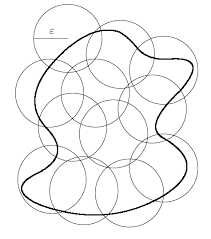
\includegraphics[width=0.3\textwidth]{../Images/CoveringNumber}
%    \end{center}
%}

\end{frame}






\begin{frame}
    \frametitle{The Problem}

    \begin{itemize}
        \item {\bf Avoidance Problem}: Given $Z \subset (\RR^d)^n$, find $X \subset \mathbf{R}^d$ with large dimension such that for distinct points $x_1, \dots, x_n \in X$, $(x_1, \dots, x_n) \not \in Z$. We say $X$ \emph{avoids} $Z$.

        \pause
        \item Let $Z = \{ (x,y,z) \in (\RR^d)^3: (x - z) \cdot (y - z) = 0 \}$.
        %
        \begin{itemize}
            \item $X \subset \RR^d$ avoids $Z$ iff $X$ does not contain any right angles.
        \end{itemize}

%        \item For each $m \in \ZZ^n - \{ 0 \}$ and $a \in \ZZ$, define
        %
%        \[ Z(m,a) = \{  (x_1, \dots, x_n) \in (\RR^d)^n : m_1x_1 + \dots + m_nx_n = a \}. \]
        %
%        \pause
%        If $Z_n = \bigcup_{m \in \ZZ^n - \{ 0 \}} \bigcup_{a \in \ZZ} Z(m,a)$, then $X \subset \RR^d$ avoids $Z_n$ for all $n > 0$ if and only if $X$ generates a subgroup of $\RR^d$ disjoint from $\QQ^d - \{ 0 \}$.

        \pause
        \item How does the geometry of $Z$ help us?

        \pause
        \item e.g. $Z$ is a degree $2$ algebraic hypersurface in last example.
    \end{itemize}
\end{frame}




\begin{frame}
    \frametitle{Results in Literature}

    \begin{itemize}
        \pause
        \item Math\'{e} (2012): If $Z \subset (\RR^d)^n$ is an algebraic hypersurfaces specified by a rational coefficient polynomial with degree at most $r$, then we can $X \subset \RR^d$ avoiding $Z$ with
        %
        \[ \hausdim(X) = d/r. \]

        \pause
        \item Fraser and Pramanik (2016): If $Z \subset (\RR^d)^n$ is a smooth hypersurface with dimension at most $m$, we can find $X \subset \RR^d$ avoiding $Z$ with
        %
        \[ \hausdim(X) = \frac{nd-m}{n-1}. \]

        \pause
        \item What if we use less rigid geometric information, i.e. the fractal dimension of the set Z?
    \end{itemize}
\end{frame}

\begin{frame}
    \frametitle{Our Results}

    \begin{itemize}
        \item D, Pramanik, and Zahl (2019): If $Z \subset (\RR^d)^n$ is a set with Minkowski dimension bounded by $s$, we can find $X \subset \RR^d$ avoiding $Z$ with
        %
        \[ \hausdim(X) = \frac{nd-s}{n-1}. \]

        \pause
        \item D (2019): If $Z \subset \RR^n$, and $\pi: \RR^n \to \RR^m$ is a rational coefficient projection map such that $\pi(Z)$ has Minkowski dimension bounded by $s$, then we can find $X \subset \RR$ avoiding $Z$ with
        %
        \[ \hausdim(X) = \frac{m - s}{m}. \]
    \end{itemize}
\end{frame}





\begin{frame}
    \frametitle{Applications}

    \begin{itemize}
        \item Given a subgroup $H \subset \RR$, is it possible to find $G \subset \RR$ such that $G + H = \RR$?

        \pause
        \item \textbf{Theorem:} Let $H \subset \RR$ be a set with Minkowski dimension $s$. Then we can find an additive subgroup $G \subset \RR$ such that $G \cap H \subset \{ 0 \}$ and such that $\hausdim(G) = 1-s$.

        \begin{itemize}
            \item It seems likely that whatever higher dimensional generalization of our results should construct $G \subset \RR^d$ with Hausdorff dimension $d - s$ for any group $H$ of Minkowski dimension $s$.
        \end{itemize}
    \end{itemize}
\end{frame}







\begin{frame}
    \frametitle{Applications}

    \begin{itemize}
        \item Since we use `rough' geometric information about $Z$, our method can even consider `avoidance problems on fractals'.

        \pause
        \begin{itemize}
            \item Consider the Cantor dust $E$, with $\minkdim(E) = 1$.

            \pause
            \item If $\pi: E \to \RR$ is a projection onto the line at a $45^{\circ}$ angle, $\pi(E)$ is an interval.

            \pause
            \item Let
            %
            \[ Z = \left\{ (x,y,z) \in \pi(E)^3 : \begin{array}{c}
            \text{there is $x_0, y_0, z_0 \in E$}\\
            \text{s.t. $(x_0 - z_0) \cdot (y_0 - z_0) = 0$}
        \end{array} \right\}. \]

            \pause
            \item Basic considerations suggest that $\minkdim(Z) = 2$, so that we can find $X \subset \pi(E)$ avoiding $Z$ with Haudsorff dimension $1/2$.

            \pause
            \item Then $\pi^{-1}(X)$ avoids right angles and $\hausdim(\pi^{-1}(X)) \geq 1/2$.
        \end{itemize}

        \pause
        \item (D, Pramanik, Zahl, 2019) used this technique to bound the existence of isosceles triangles on Lipschitz curves.
    \end{itemize}
\end{frame}

\begin{frame}

\begin{center}
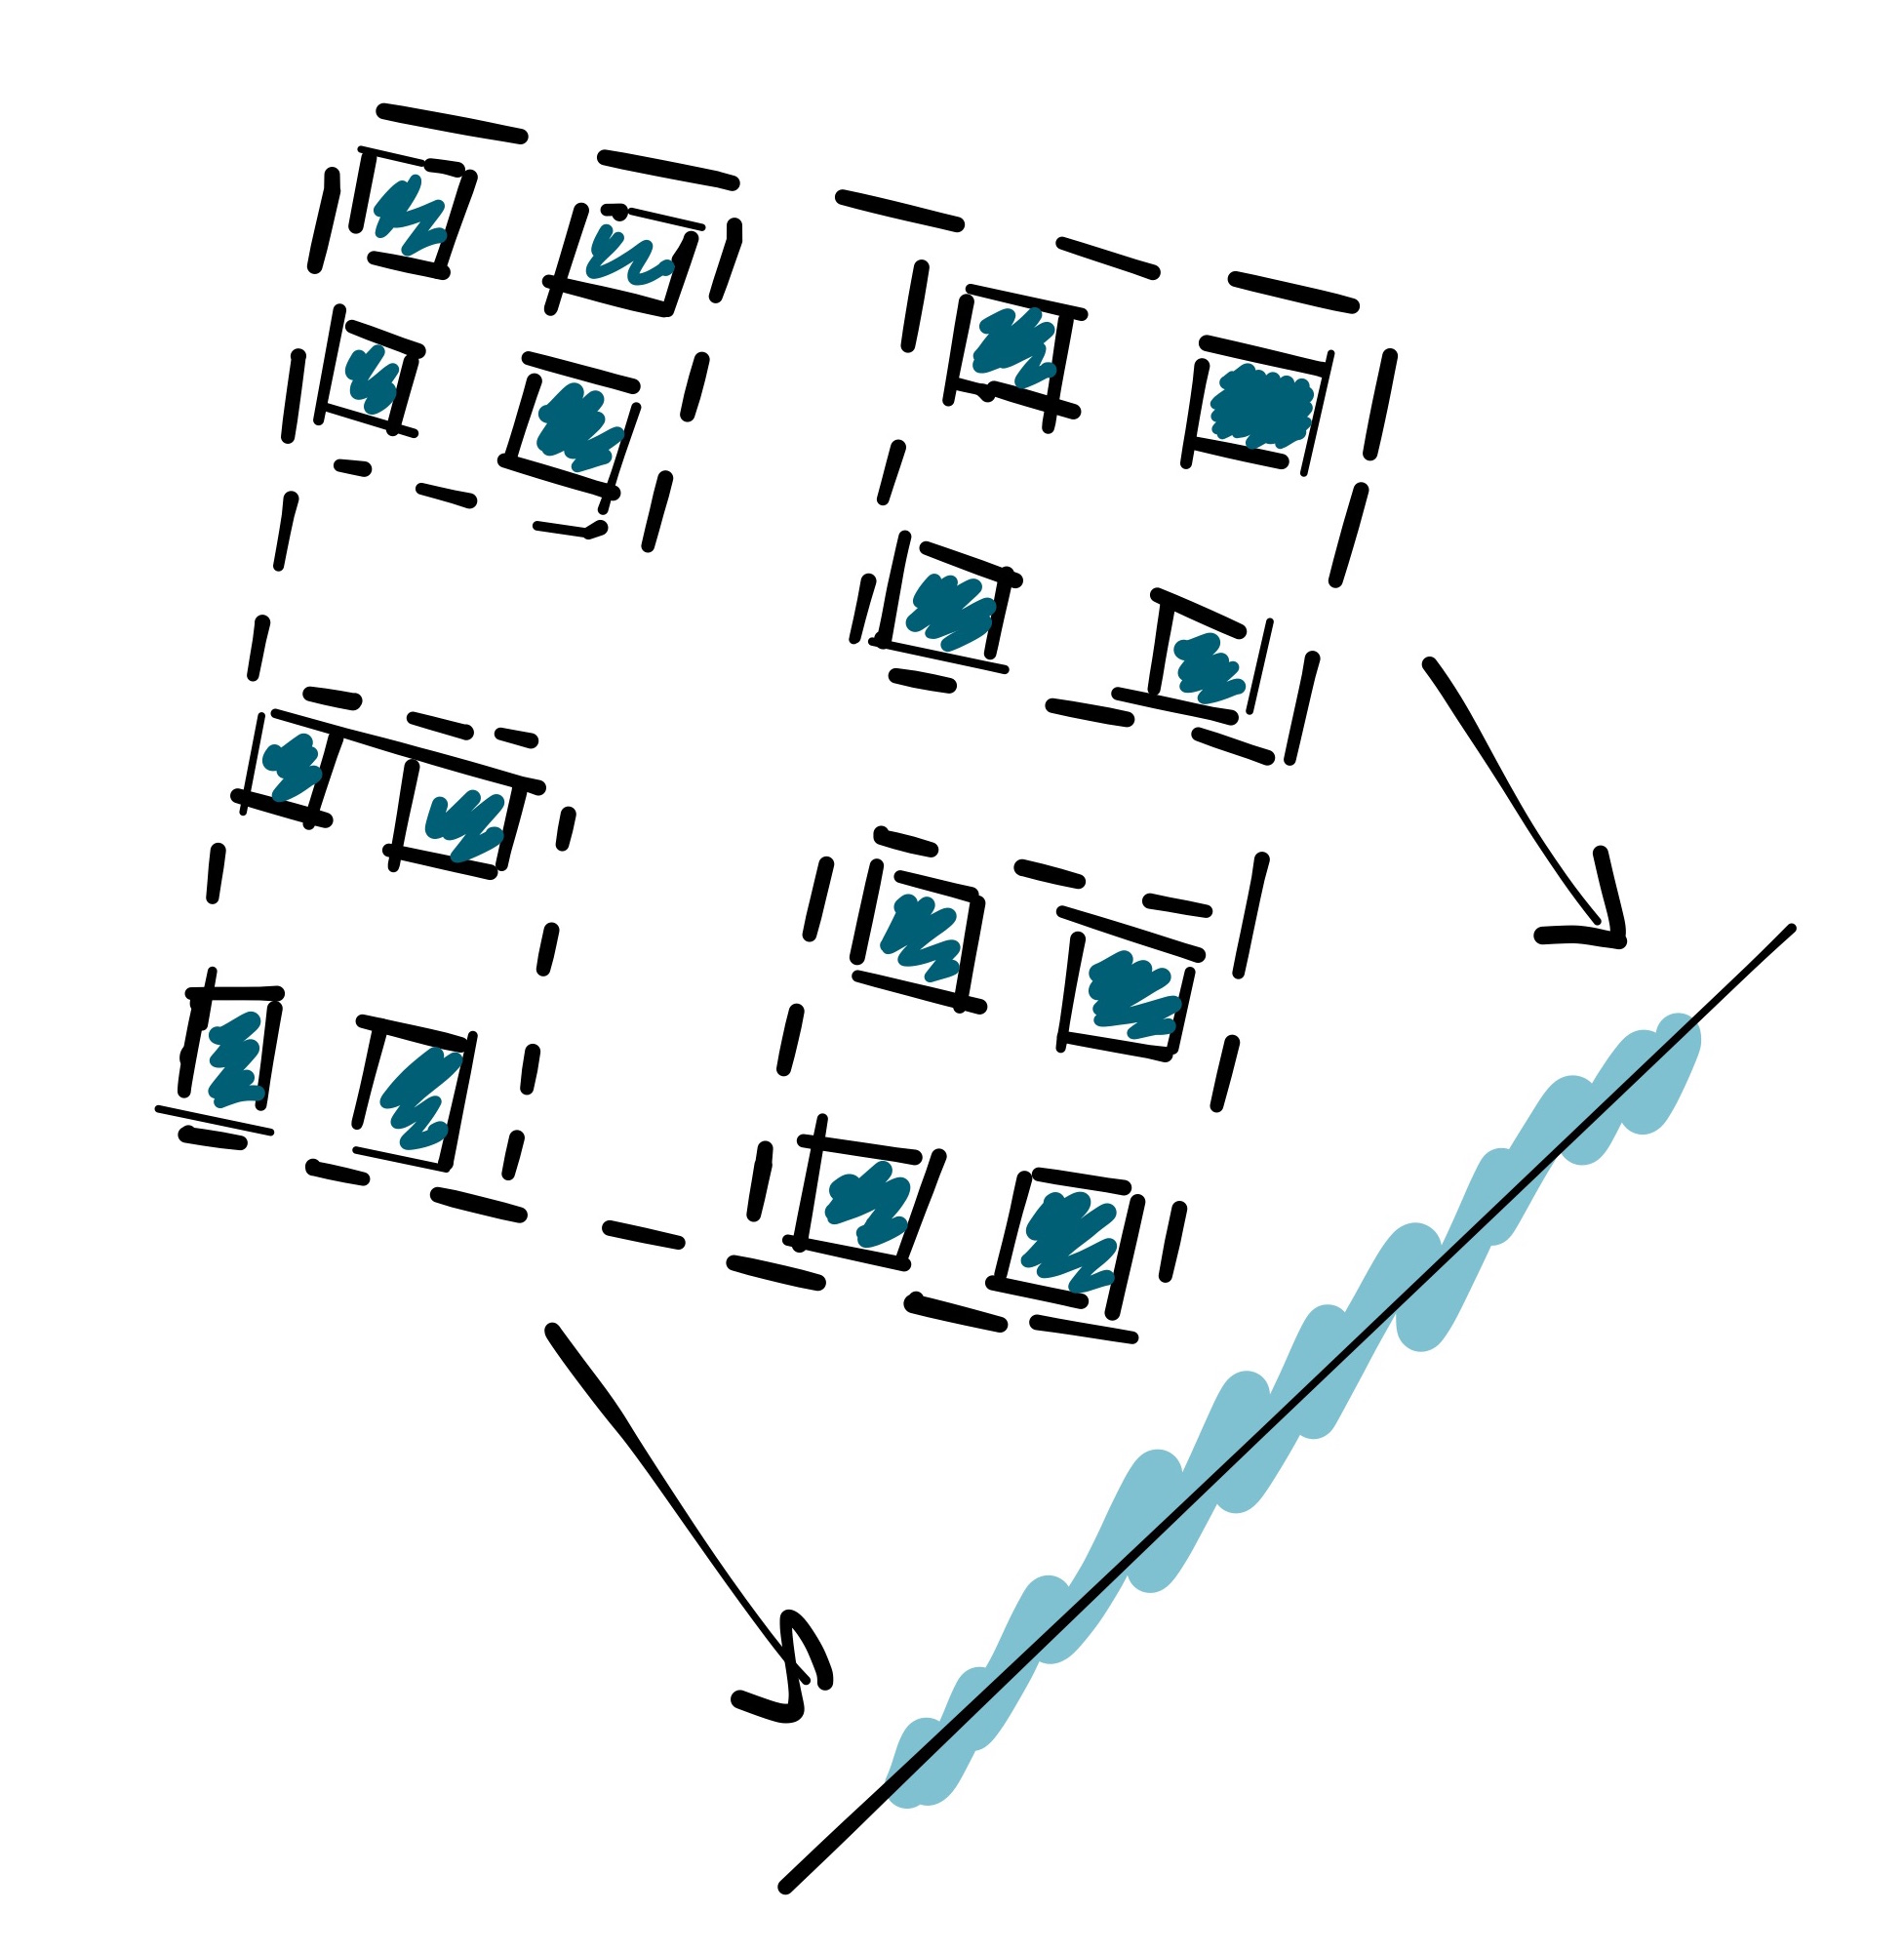
\includegraphics[width=0.8\textwidth]{../Images/CantorDustProjection}
\end{center}

\end{frame}





\begin{frame}
    \frametitle{Fourier Dimension}

    \begin{itemize}
        \pause
        \item A set $X \subset \RR^d$ has \emph{Fourier dimension} at least $s$ if there exists a finite measure $\mu$ supported on $X$ such that $|\widehat{\mu}(\xi)| \lesssim |\xi|^{-s/2}$.

        \pause
        \item Often gives much more structural information about a set than Minkowski dimension does.

        \pause
        \item (Keleti, 1998) There exist an `independent' set $X$ with full Hausdorff dimension such that there exists no nontrivial solutions to $m_1x_1 + \dots + m_nx_n = 0$ for any $m \in \ZZ^n$ and $x_1, \dots, x_n \in X$.

        \pause
        \item (Rudin, 1960) If $X$ has Fourier dimension greater than $1/n$, then there exists some $m \in \ZZ^n$ and some $x_1, \dots, x_n \in X$ such that $m_1 x_1 + \dots + m_n x_n = 0$.
    \end{itemize}
\end{frame}

\begin{frame}
    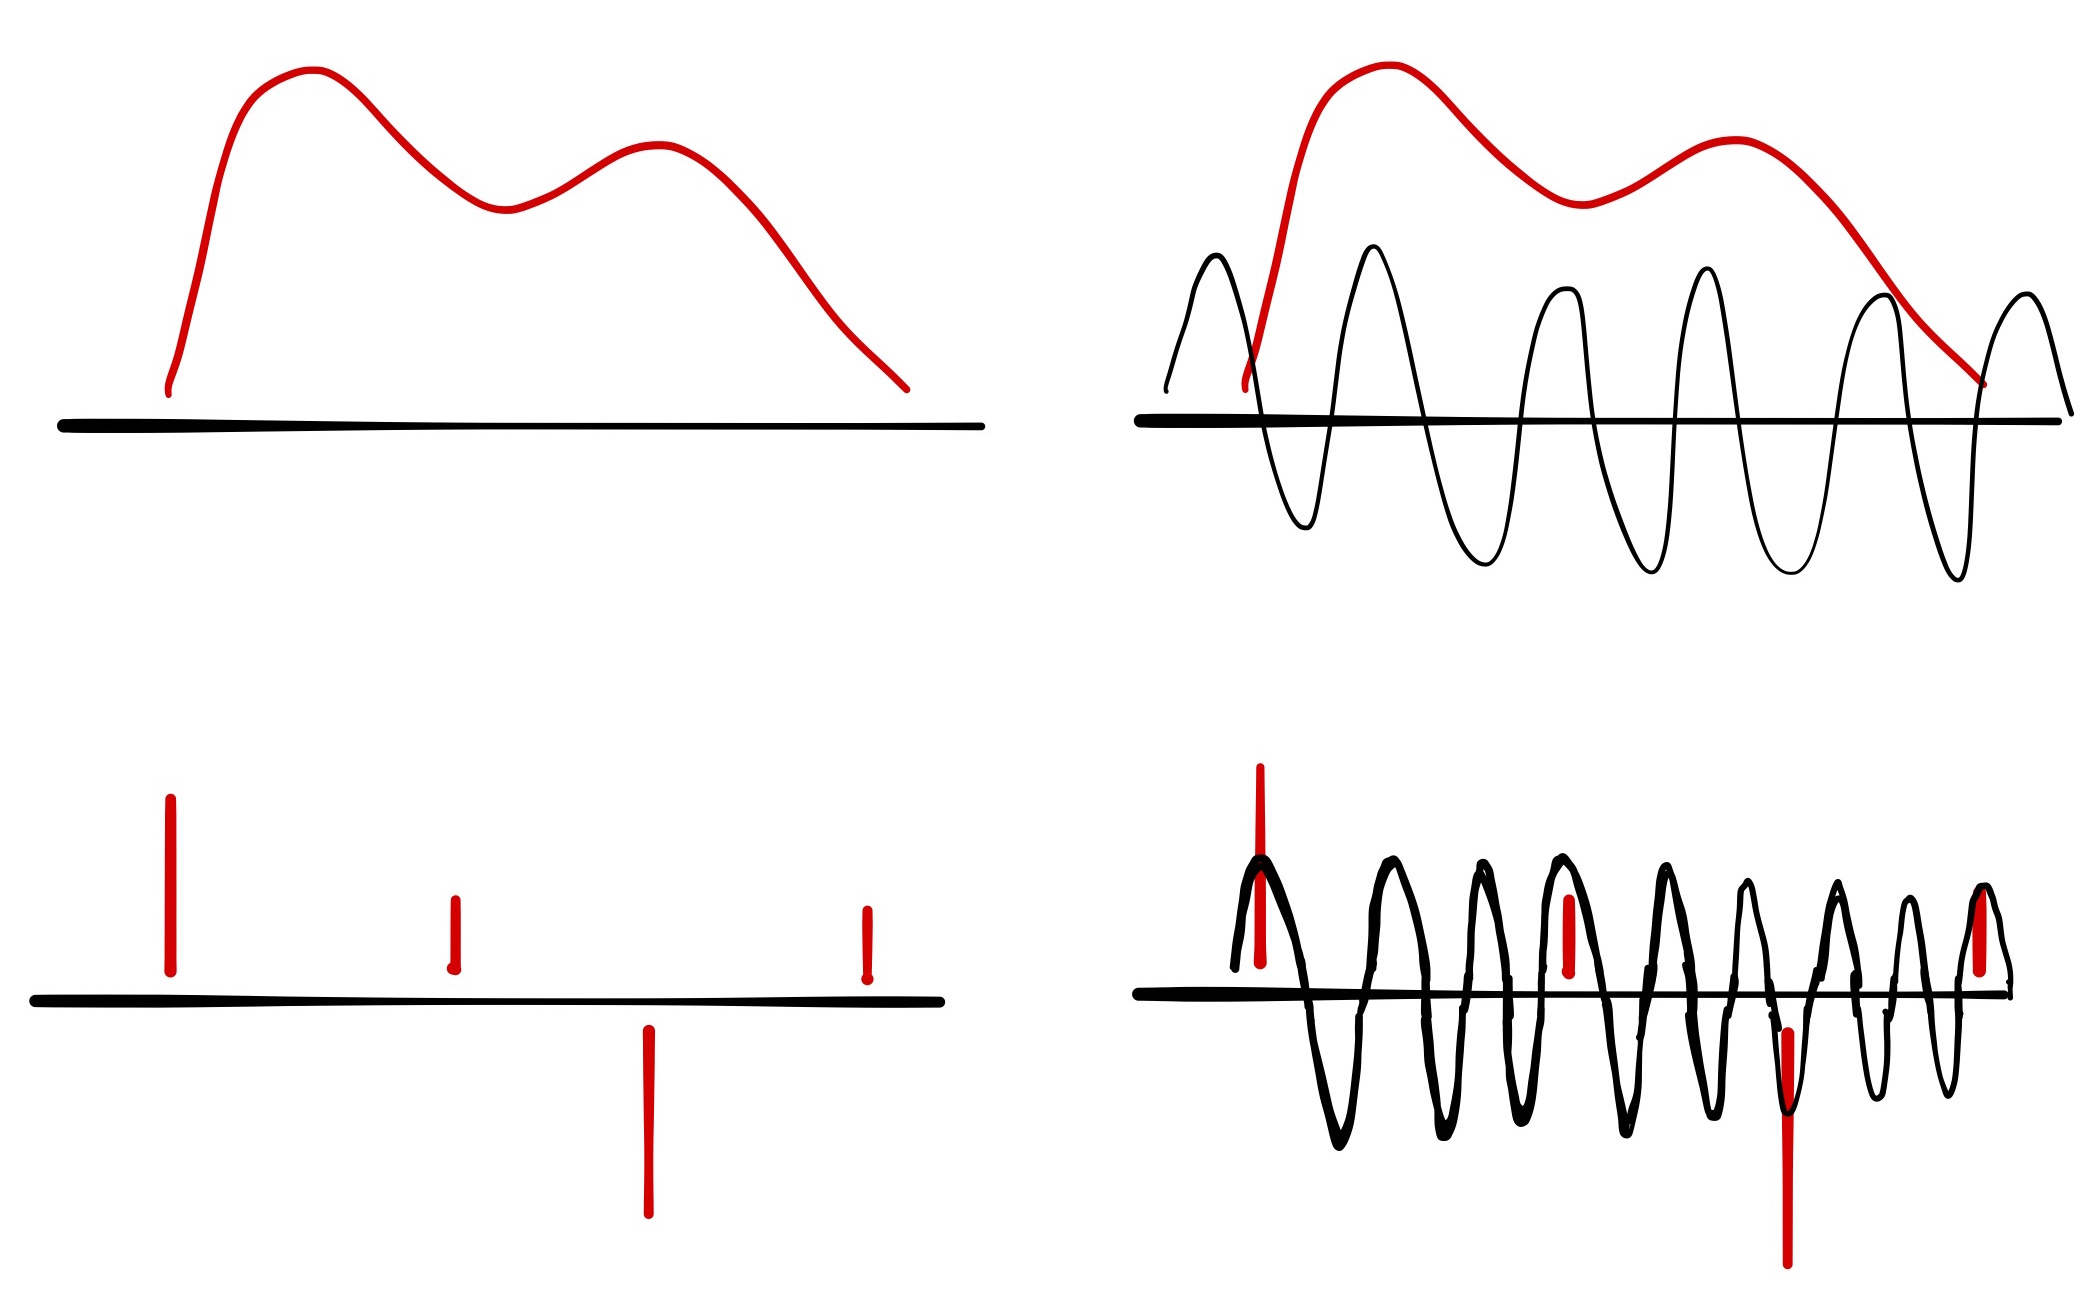
\includegraphics[width=\textwidth]{../Images/FourierDimension}
\end{frame}



\begin{frame}
    \frametitle{Getting Fourier Dimension Bounds Is Hard}

    \begin{itemize}
        \item For any set $X$, $\fordim(X) \leq \hausdim(X) \leq \minkdim(X)$.

        \pause
        \item $X$ is a \emph{Salem Set} if $\fordim(X) = \hausdim(X)$.

        \pause
        \item All sets are Salem `generically', but for most explicit constructions, the Fourier dimension is equal to zero.

        \pause
        \item If $X$ is the Cantor set, then $\hausdim(X) = \minkdim(X) = \log_3(2)$, but $\fordim(X) = 0$.

        \begin{center}
        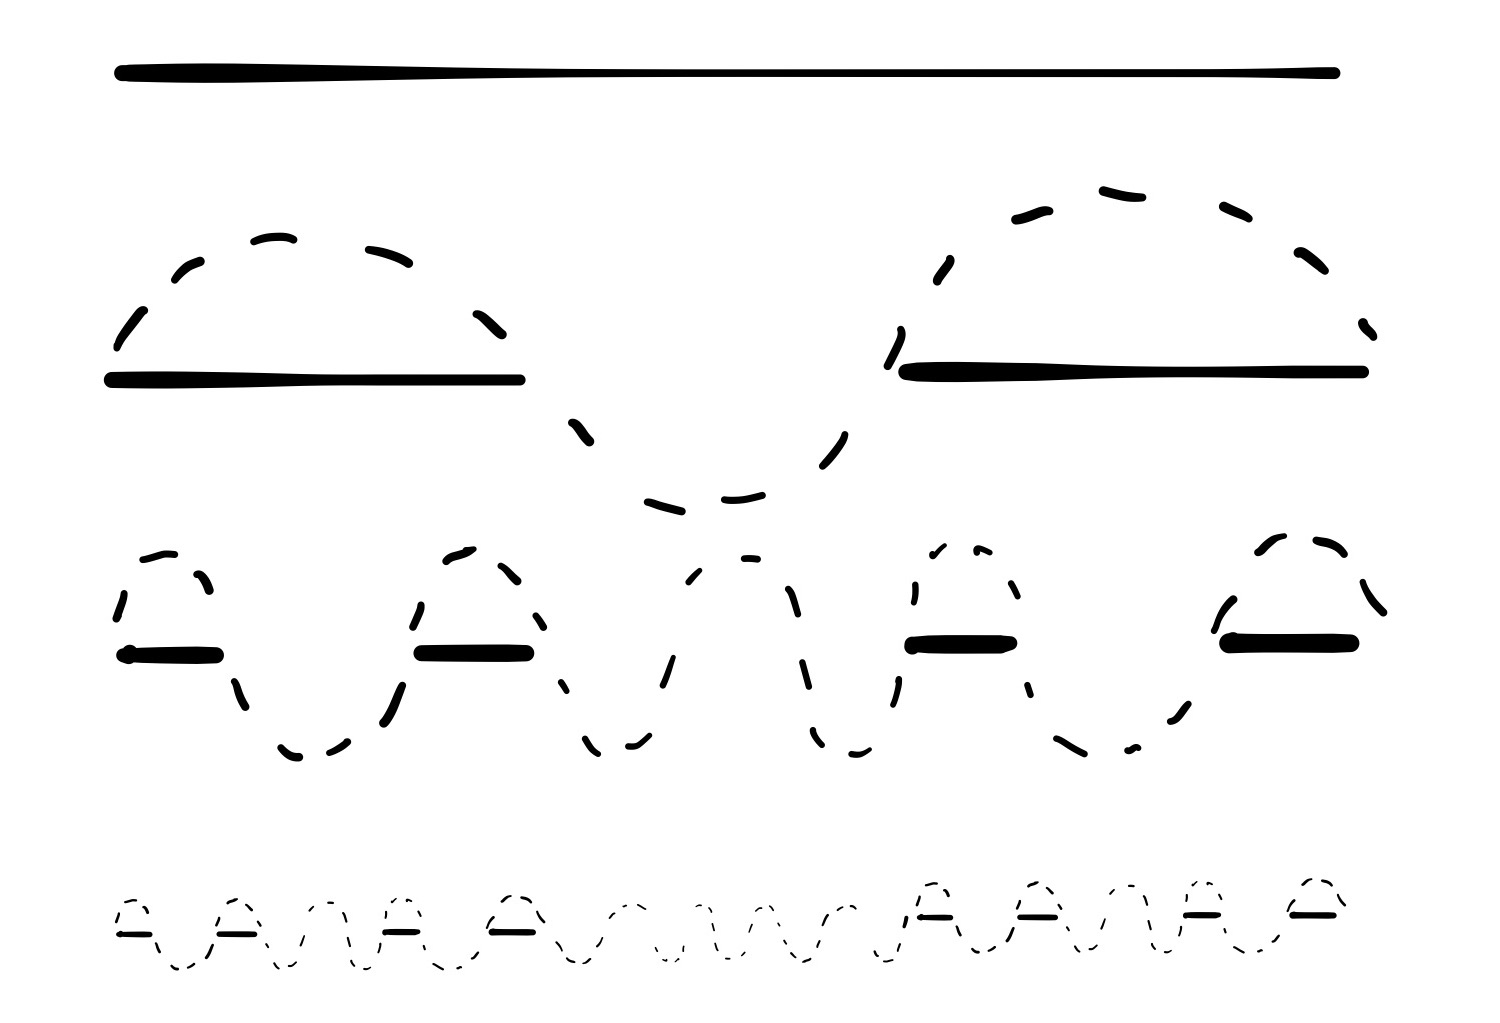
\includegraphics[width=0.5\textwidth]{../Images/CantorSetFourier}
        \end{center}

        \pause
        \item Heuristic: Typically need `square root cancellation' to obtain optimal Fourier decay, e.g. by using randomness.
    \end{itemize}
\end{frame}

%\begin{frame}
%    \frametitle{The Avoidance Problem}

%        \begin{itemize}

%            \item Our method naturally considers an equivalent setup.

%            \item {\bf Fractal Avoidance Problem}: Given $Y \subset \mathbf{R}^{nd}$, find $X \subset \mathbf{R}^d$ such that $X^n \cap Y \subset \Delta$, where $\Delta = \{ x: x_i = x_j\ \text{for some $i,j$} \}$.

%            \item Equivalent by setting $Y = f^{-1}(0)$, or $f = \mathbf{I}_{Y^c}$.

%            \item Our method only uses the structure of the zero set, not $f$.
%        \end{itemize}
%\end{frame}

\begin{frame}
    \frametitle{Salem Set Result}

    \pause
    \begin{theorem}[2021, D]
        If $Z$ has lower Minkowski dimension bounded by $s$, we can find $X$ avoiding $Z$ with
        %
        \[ \hausdim(X) = \fordim(X) = \frac{nd - s}{n - 1/2}. \]
    \end{theorem}

    \pause
    \begin{theorem}[2021, D]
        If $Z$ is the countable union of sets $Z_n$ of the form
        %
        \[ Z_n = \{ (y,x_1,\dots,x_{n-1}) \in (\RR^d)^n: y = f_n(x_1,\dots,x_{n-1}) \}, \]
        %
        where $f_n \in C^\infty((\RR^d)^n, \RR^d)$, and for $1 \leq i \leq n-1$, $D_{x_i} f_n$ is an invertible matrix, then we can find $X$ avoiding $Z$ with
        %
        \[ \hausdim(X) = \fordim(X) = \frac{d}{n-3/4}. \]
    \end{theorem}
\end{frame}






\begin{frame}
    \begin{itemize}
        \item D, Pramanik, and Zahl (2019): If $Z \subset (\RR^d)^n$ is a set with Minkowski dimension bounded by $s$, we can find $X \subset \RR^d$ avoiding $Z$ with
        %
        \[ \hausdim(X) = \frac{nd-s}{n-1}. \]

                \pause
        \item Fraser and Pramanik (2016): If $Z \subset (\RR^d)^n$ is a smooth hypersurface with dimension at most $m$, we can find $X \subset \RR^d$ avoiding $Z$ with
        %
        \[ \hausdim(X) = \frac{nd-m}{n-1}. \]
    \end{itemize}
\end{frame}





\begin{frame}

\begin{center}
    {\huge Thanks for listening!}
    \\
    \\
    {If you're interesting in hearing more, contact me at \href{jcdenson@wisc.edu}{jcdenson@wisc.edu}.}
    \ 
\end{center}

\end{frame}

\end{document}